\documentclass{beamer}
% \usepackage[utf8]{inputenc}
\usepackage{default}
\mode<presentation>{
    %\usepackage{beamerthemeshadow}
    %\usepackage{beamerthemeshadow}
    %\usepackage{beamerthemePaloAlto}
    %\usepackage{beamerthemeSzeged}
    %\usepackage{beamerthemeAntibes}
    %\usepackage{beamerthemeBergen}
    %\usepackage{beamerthemeBerkeley}
    %\usepackage{beamerthemeBerlin}
    %\usepackage{beamerthemeBoadilla}  
    %\usepackage{beamerthemeboxes}  
    %\usepackage{beamerthemeCambridgeUS}
    %\usepackage{beamerthemeCopenhagen} 
    %\usepackage{beamerthemeDarmstadt}
    %\usepackage{beamerthemeDresden}
    %\usepackage{beamerthemeFrankfurt}
    %\usepackage{beamerthemeGoettingen}
    %\usepackage{beamerthemeHannover}
    \usepackage{beamerthemeIlmenau}
    %\usepackage{beamerthemeJuanLesPins} 
    %\usepackage{beamerthemeLuebeck} 
    \usepackage{pgf,pgfarrows,pgfnodes,pgfautomata,pgfheaps,pgfshade}
    \usepackage{clrscode3e}
    \beamertemplatetransparentcovereddynamic
    \beamertemplateballitem
    %\beamertemplatefootpagenumber
}
\mode<handout>{
    \usepackage[bar]{beamerthemetree}
    % Colocando um fundo cinza quando for gerar transparências para serem impressas
    % mais de uma transparência por página
    \beamertemplatesolidbackgroundcolor{black!5}
}
% \usepackage[ruled,chapter]{algorithm}
\usepackage{algorithm}	
\usepackage{algorithmic}

\usepackage{comment}
\usepackage{amsmath,amssymb}
\usepackage[brazil]{varioref}
\usepackage[english,brazil]{babel}
\usepackage[utf8]{inputenc}
\usepackage{graphicx}
\usepackage[alf]{abntex2cite}
\usepackage{abntex2abrev}
% \usepackage[round,sort,authoryear,nonamebreak]{natbib}
% \usepackage[authoryear]{natbib}
%\usepackage{minitoc-hyperref}
%\usepackage{listings}
%\usepackage{listings}
%\usepackage{colortbl}
%\usepackage{pslatex}
\beamertemplatetransparentcovereddynamic

\usepackage{tikz}
\usetikzlibrary{arrows}
\tikzstyle{block}=[draw opacity=0.7,line width=1.4cm]

\newcommand*\oldmacro{}%
\let\oldmacro\insertshorttitle%
\renewcommand*\insertshorttitle{%
  \oldmacro\hfill%
  \insertframenumber\,/\,\inserttotalframenumber}

\title[Trabalho de Conclusão de Curso]{Trabalho de Conclusão de Curso}
\subtitle{Desenvolvimento de um sistema web para a Associação dos Protetores da Bacia hidrográfica do Rio Gorutuba ``Kuruatuba''}

%\titlegraphic{}

\author[Guilherme Rocha Leite]{Guilherme Rocha Leite}
  \institute[UFVJM]{Universidade Federal dos Vales do Jequitinhonha e Mucuri \newline
  Bacharelado em Sistemas de Informação \newline
%   \inst{Departamento de Computação
	  
     Orientador: Prof.ª Erinaldo Barbosa da Silva\\
     Co-orientador: Thales Francisco Mota Carvalho\\
     $~$\\
%      Disciplina: Nome da Disciplina\\
}
\logo{
\includegraphics[scale=0.1]{logo-ufvjm.jpg}}
% Se comentar a linha abaixo, irá aparecer a data quando foi compilada a apresentação
%\date{\textcolor{red}{III Encontro Mineiro de Equações Diferenciais, 2009}}
%\pgfdeclareimage[height=0.4cm]{das}{figs/logodas}
%\pgfdeclareimage[height=1cm]{logo}{logos}
% pode-se colocar o LOGO assim
%\logo{\pgfuseimage{logo}}
% ou...
%\logo{\vbox{\hbox to 3cm{\hfil\pgfuseimage{logo}}}}

\begin{document}
%\xdefinecolor{MyGreen}{rgb}{0,0.6,0}
%\beamerboxesdeclarecolorscheme{MyGreen}{MyGreen}{MyGreen!20!averagebackgroundcolor}
\beamerboxesdeclarecolorscheme{formula}{white}{blue!250!averagebackgroundcolor}
\frame{\titlepage}

%\frame{\titlepage}
\part{Presentation}
% \section{Sumário}

\frame{
\frametitle{Sumário}
\tableofcontents
}

\AtBeginSection[]{
  \frame<handout:0>{
    %\frametitle{Sumário}
    \tableofcontents[current,currentsection]
  }
}

%===================================Slide=================================================

\section{Introdução}

\begin{frame}
    \frametitle{Sobre a Kuruatuba}
    \begin{itemize}
        \item \textbf{Fundação:} 1989 - Associação de Futebol de Praia do Copo Sujo de Janaúba;
        \item \textbf{Objetivo:} promoção de esporte, lazer, cultura e preservação e conservação da Bacia do Rio Gorutuba;
        \item \textbf{Parcerias:} Secretaria de Meio Ambiente da Prefeitura de Janaúba e Ruralminas, IEF, CODEMA, Poder Judiciário (Albergados), escolas, igrejas e outros segmentos;
        \item \textbf{Criação do estatuto:} 2003.
    \end{itemize}

\end{frame}


%pag 20
%justificativa 
\begin{frame}
    \frametitle{Motivação}
    \textbf{Principais dificuldades:}
    \begin{itemize}
     \item Impulsionar publicações e atrair apoiadores;
     \item Gerenciar pessoas e arquivos digitais relacionadas à associação.
    \end{itemize}

    
    \textbf{Problemas encontrados:}
    \begin{itemize}
        \item Informalidade em utilização de blog: opiniões pessoais para assuntos específicos \cite{centeno2017pampatur};
        \item Baixos controle de usuários e personalização visual de um blog; %não tem tanto nível hierárquico entre administradores
        \item Baixa capacidade de atingir o público alvo em publicações; %apenas 7,1% recebem notícias via site ou blog e 56,3% gostariam
        \item Dificuldade em manter membros e associados registrados e atualizados.
    \end{itemize}

\end{frame}


%pag 21
\begin{frame}
    \frametitle{Objetivos}
    \textbf{Objetivo geral:} construção de um sistema web para auxiliar na gestão das informações e propagação de conteúdo de autoria da Kuruatuba.
    
    \textbf{Objetivos específicos:}
    \begin{itemize}
        \item Oferecer manutenção, segurança e disponibilidade das informações;
        \item Promover divulgação de vários tipos de conteúdo de maneira organizada;
        \item Possibilitar o gerenciamento de pessoas e administradores vinculados à Kuruatuba;
        \item Aprofundar estudos sobre engenharia e desenvolvimento de software e segurança de dados.
    \end{itemize}
\end{frame}


%pags 24 e 28
%Pra que CMS e Metodologias de desenvolvimento
\section{Desenvolvimento}
\begin{frame}
    \frametitle{Escolha de Métodos e Ferramentas}
    \textbf{Motivos para usar alguma metodologia ágil:} \cite{dos2013metodologias}
    \begin{itemize}
        \item Tempo: Cronograma orientado a produto com entregas incrementais (entregas por partes);
        \item Custo: Maior controle em função da rapidez em alterações; %alterações realizadas em tempo real de acordo com o feedback do cliente
        \item Definição inicial: tempo em \textit{sprints}.
    \end{itemize}
    
\end{frame}

\begin{frame}
 \frametitle{Escolha de Métodos e Ferramentas}
 %pag 41
    \textbf{Motivos para a escolha do \textit{Scrum}:} \cite{anwer2017comparative}
    \begin{itemize}
        \item Elicitação de requisitos: Não definido (à escolha da equipe); %fica a critério da equipe como coletar os requisitos
        \item Ordem de desenvolvimento definida pela equipe \textit{Scrum}; %a equipe tem liberdade de definir quais serão as etapas de desenvolvimento e o prazo para cada uma
        \item Tamanho da equipe: de 1 a 10 indivíduos. %ficando possível ser realizado com 1 indivíduo
    \end{itemize}
\end{frame}



\begin{frame}
    \frametitle{Escolha de Métodos e Ferramentas}
    \textbf{Motivos para usar algum Sistema de Gerenciamento de Conteúdo (CMS):} (\citeonline{meike2009security}; \citeonline{chagas2018estudo})
    \begin{itemize}
        \item Possibilidade de múltiplos usuários gerenciarem um website ou portal simultaneamente;
        \item Redução de erros de publicação; %O CMS contém os campos necessários que devem ser preenchidos para uma publicação qualquer 
        \item Sem necessidade de conhecimento em programação; %usuários podem manusear sem precisar saber programar
        \item Possibilidade de se definir nı́veis de acesso a usuários por grupo. %é possível definir quais partes do sistema cada usuário poderá gerenciar
    \end{itemize}
\end{frame}

\begin{frame}
    \frametitle{Escolha de Métodos e Ferramentas}
    %pag 49
    \textbf{Motivos para a escolha do Plone:}
    \begin{itemize}
        \item Apropriado para construção de portais (a exemplo do portal da UFVJM e do portal do governo federal);
        \item Sem necessidade de instalação de \textit{plug-ins} adicionais; %que, inclusive, podem afetar o desempenho e a manutenibilidade de um sistema por alta quantidade de plug-ins
        \item Segurança fornecida pela combinação do \textit{Plone} com o \textit{Zope}. %que é o servidor de banco de dados que o Plone utiliza
    \end{itemize}
\end{frame}


\begin{frame}
    \frametitle{Escolha de Métodos e Ferramentas}
    
    \begin{figure}[htb]
        \centering
        \caption{Desempenho obtido pelo \textit{Plone}. Fonte: \cite{elias}.}
        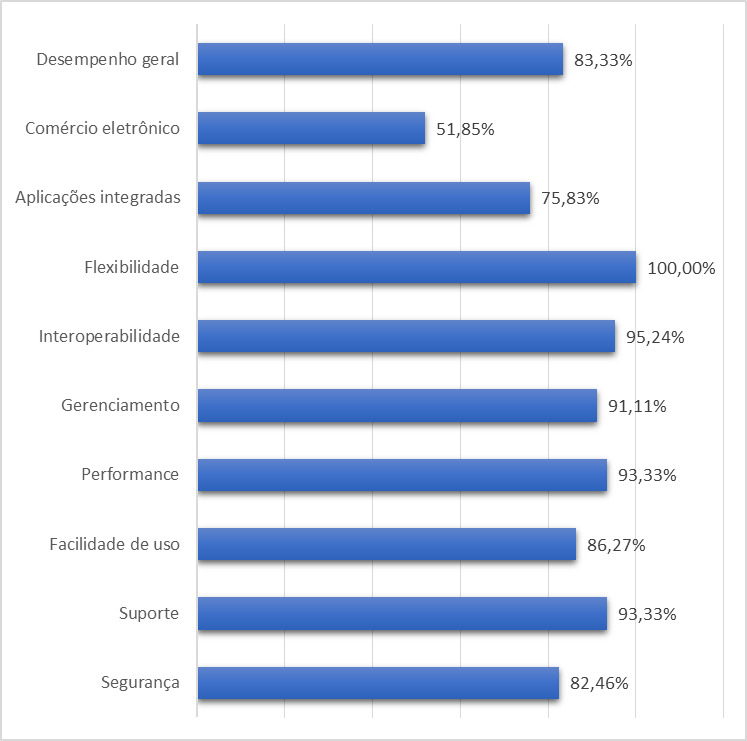
\includegraphics[width=0.5\textwidth]{../figuras/desempenho-plone}
        \label{plone}
    
    \end{figure}
    
\end{frame}


\begin{frame}
    \frametitle{Escolha de Métodos e Ferramentas}
    
    %A título de comparação com um CMS conhecido...
    \begin{figure}[htb]
        \centering
        \caption{Desempenho obtido pelo \textit{WordPress}. Fonte: \cite{elias}.}
        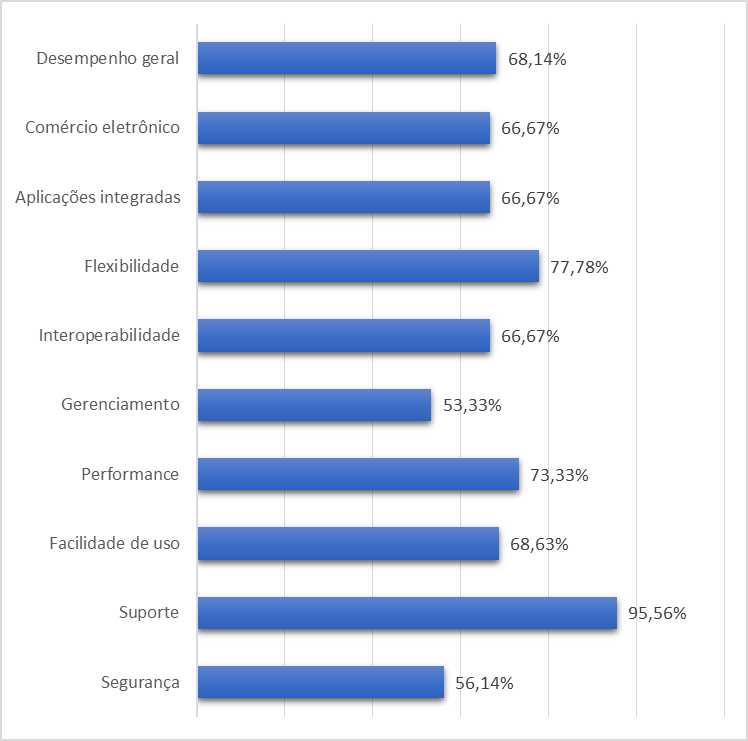
\includegraphics[width=0.5\textwidth]{../figuras/desempenho-wordpress}
        \label{wordpress}
    \end{figure}
        
\end{frame}


%pag 40
\begin{frame}
    \frametitle{Outras Ferramentas Utilizadas}
    \textbf{\textit{Docker}:} 
    \begin{itemize}
        \item Surgimento em 2013;
        \item Estrutura em imagens, camadas e ``containers'';
        \item Vantagens: escalabilidade (fragmentação de todo o sistema em partes), indepedência entre ``containers'', portabilidade (facilidade em executar o sistema em ambientes diferentes) e verificação de erros via relatório de \textit{logs}. 
    \end{itemize}
    
\end{frame}

\begin{frame}
    \frametitle{Outras Ferramentas Utilizadas}
    \textbf{\textit{Git}:} 
    \begin{itemize}
        \item Surgimento em 2005;
        \item Utilizado para versionamento de código; %consegue acompanhar e retornar à versões anteriores
        \item Vantagens: gerenciar versionamento de código, desenvolver aplicações em colaboração e possibilidade de manter código privado quando manuseado com um site de hospedagem de códigos.
    \end{itemize}
\end{frame}


\begin{frame}
    \frametitle{Outras Ferramentas Utilizadas}
    \textbf{\textit{Google Analytics}:} 
    \begin{itemize}
        \item Objetivo: obtenção de relatório com dados sobre visitantes de um website;
        \item Vantagens: identificação de padrões relacionados a visitantes, como origem e número de acessos, conteúdos acessados e tempo de duração de cada sessão. %sendo um grande medidor do impacto dos conteúdos publicados e seu alcance
    \end{itemize}
\end{frame}


\begin{frame}
    \frametitle{Outras Ferramentas Utilizadas}
    \textbf{MySQL:} 
    \begin{itemize}
        \item Tipo de Sistema Gerenciador de Bancos de Dados (SGBD) que atua com bancos de dados relacionais; %bancos que atuam com relacionamentos entre tabelas
        \item Vantagens: possui todos os atributos necessários a um banco de dados de grande porte \cite{milani2007mysql}, possui código aberto e de fácil utilização. 
    \end{itemize}
    
\end{frame}



%pag 54
\begin{frame}
    \frametitle{Coleta de Requisitos}
    \textbf{Recursos utilizados:}
    \begin{itemize}
        \item Reuniões e questionários;
        \item Histórias de usuário;
        \item Diagramas de casos de uso;
        \item Fluxos de eventos.
    \end{itemize}
\end{frame}


%pag 56
\begin{frame}
    \frametitle{Diagrama de casos de uso do portal da Kuruatuba}
    \begin{figure}[htb]
        \centering
        
        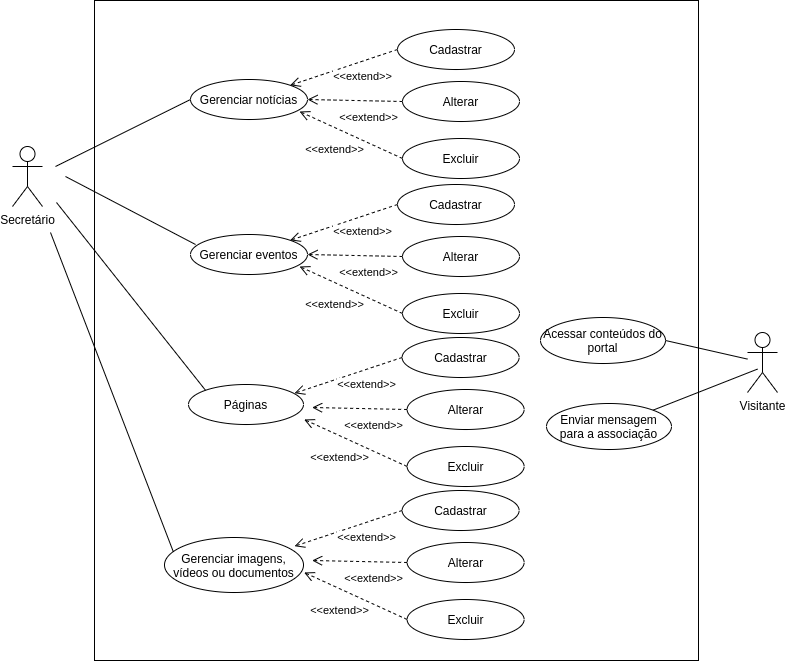
\includegraphics[width=0.7\textwidth]{figuras/use-case-portal-1.png}
        
        \label{use-case-portal}
    \end{figure}
\end{frame}

%pag 56
\begin{frame}
    \frametitle{Diagrama de casos de uso do portal da Kuruatuba}
    \begin{figure}[htb]
        \centering
        
        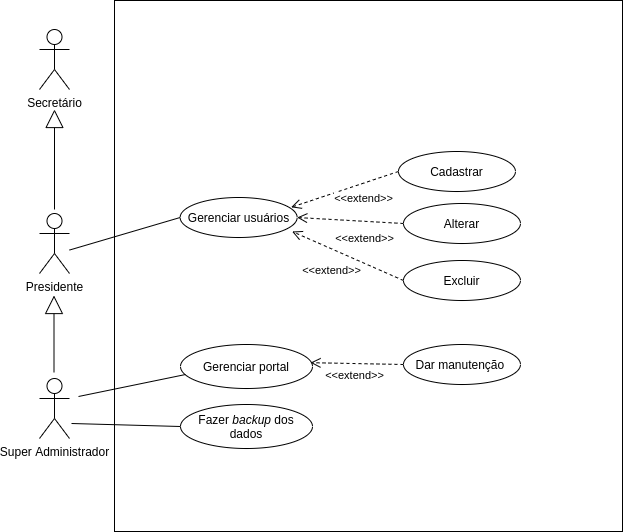
\includegraphics[width=0.6\textwidth]{figuras/use-case-portal-2.png}
        
        \label{use-case-portal}
    \end{figure}
\end{frame}

\begin{frame}
    \frametitle{Diagrama de casos de uso do sistema de associados da Kuruatuba}
    \begin{figure}[htb]
        \centering
        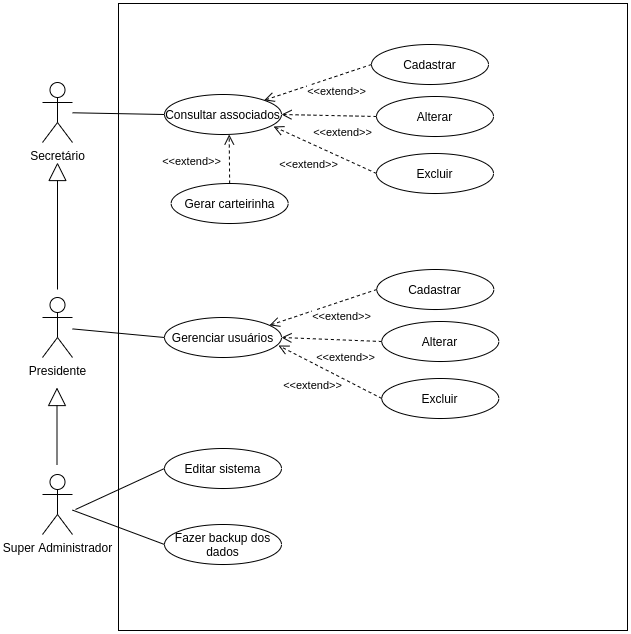
\includegraphics[width=0.56\textwidth]{../figuras/use-case-sistema.png}
        
        \label{use-case-sistema}
    \end{figure}
\end{frame}



%pag 74
\begin{frame}
    \frametitle{\textit{Product Backlog}}
    \begin{table}[h]
        \centering
        \caption{\textit{Product Backlog}. Fonte: Autor.}
        
        \resizebox{\columnwidth}{!}{ %coloca toda a tabela dentro do slide
            \begin{tabular}{c|c|c|c}
                
                \textbf{Nome} & \textbf{Tarefas} & \textbf{Prioridade} & \textbf{Prazo (dias)} \\ % Note a separação de col. e a quebra de linhas
                \hline                               % para uma linha horizontal
                
                \textit{Sprint 1} & Criação da interface inicial & 5 & 14  \\
                \rule{0pt}{13pt}
                \textit{Sprint 2} & Contratação e configuração do ambiente de desenvolvimento & 5 & 11  \\ 
                \rule{0pt}{13pt}
                \textit{Sprint 3} & Migração do portal e do sistema de associados para o servidor & 5 & 6  \\
                \rule{0pt}{13pt}
                \textit{Sprint 4} & Configuração do banco de dados e sua conexão com o sistema & 4 & 3  \\
                \rule{0pt}{13pt}
                \textit{Sprint 5} & Criação do sistema de autenticação com criptografia & 2 & 5  \\
                \rule{0pt}{13pt}
                \textit{Sprint 6} & Organização da página inicial do portal & 5 & 6  \\
                \rule{0pt}{13pt}
                \textit{Sprint 7} & Inserção de informações nas páginas & 5 & 20  \\ 
                \rule{0pt}{13pt}
                \textit{Sprint 8} & Ajustes no CRUD de associados e administradores & 3 & 6  \\
                \rule{0pt}{13pt}
                \textit{Sprint 9} & Criação do sistema de recuperação de senha e do \textit{slider} da galeria & 3 & 5  \\
                \rule{0pt}{13pt}
                \textit{Sprint 10} & Configuração do \textit{Google Analytics} e ajustes gerais & 2 & 6 \\
                
                \hline
            \end{tabular}
        }
        \label{lista-sprints}
    \end{table}
\end{frame}


%Só se achar que tem tempo pra falar:
%pag 76
% \begin{frame}
%     \frametitle{Estrutura de \textit{containers} do sistema}
%     \begin{itemize}
%         \item \textbf{Docker}
%         \item \textbf{Git}
%     \end{itemize}
% \end{frame}


%pag 79
\section{Resultados}
\begin{frame}
    \frametitle{Apresentação das Telas: Tela de Login do Portal}
    \begin{figure}[htb]
        \centering
        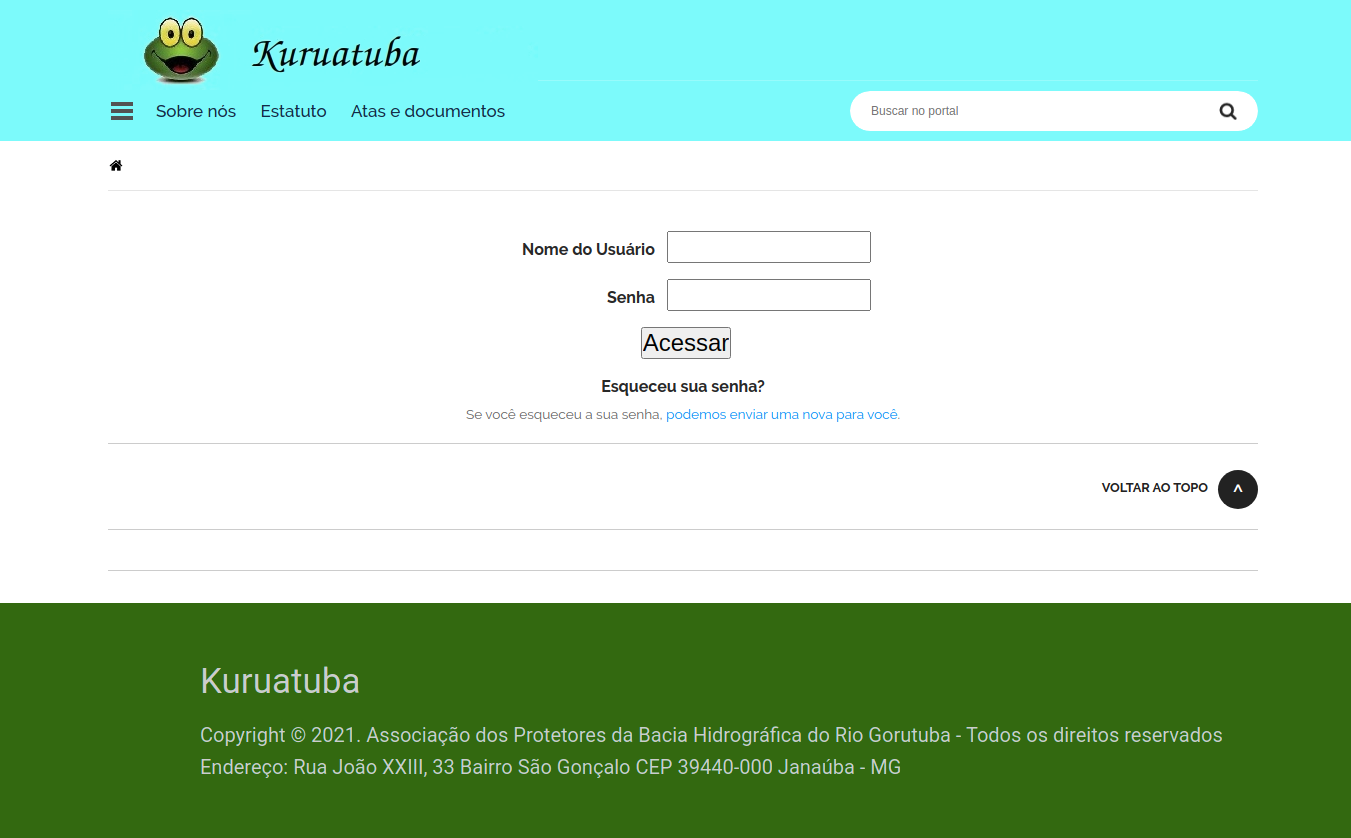
\includegraphics[width=0.9\textwidth]{../figuras/kuruatuba_portal_login.png}
        \label{fig:login-portal}
    \end{figure}
\end{frame}

\begin{frame}
    \frametitle{Apresentação das Telas: Tela de Login do Sistema de Associados}
    \begin{figure}[htb]
        \centering
        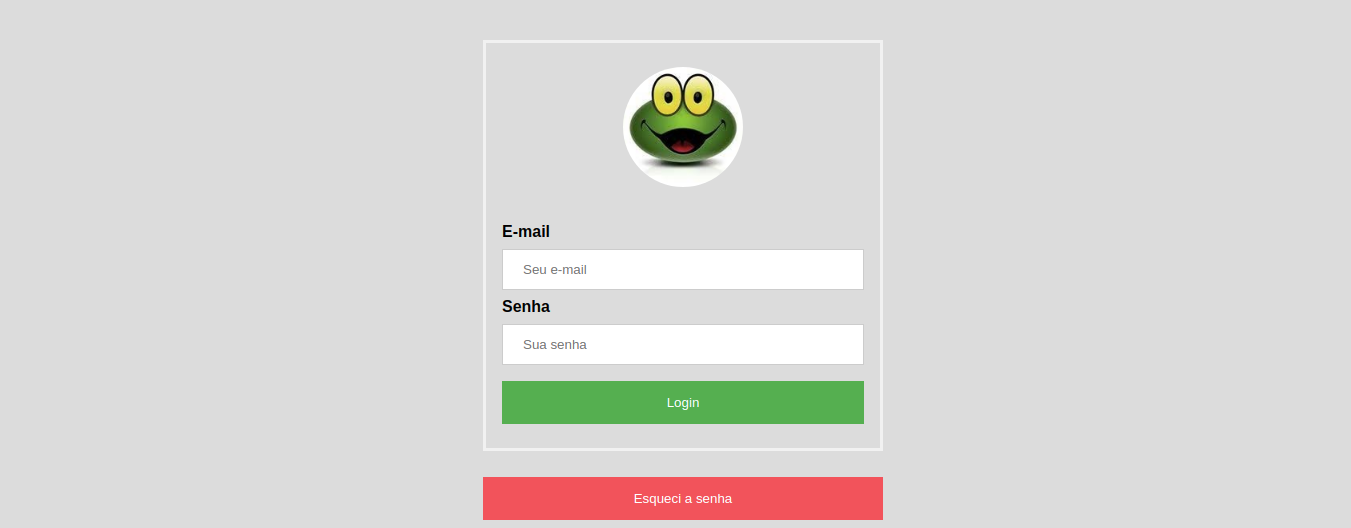
\includegraphics[width=0.9\textwidth]{../figuras/kuruatuba_sistema_login.png}
        \label{fig:login-sistema}
    \end{figure}
\end{frame}

\begin{frame}
    \frametitle{Apresentação das Telas: Página Inicial do Sistema de Associados}
    \begin{figure}[htb]
        \centering
        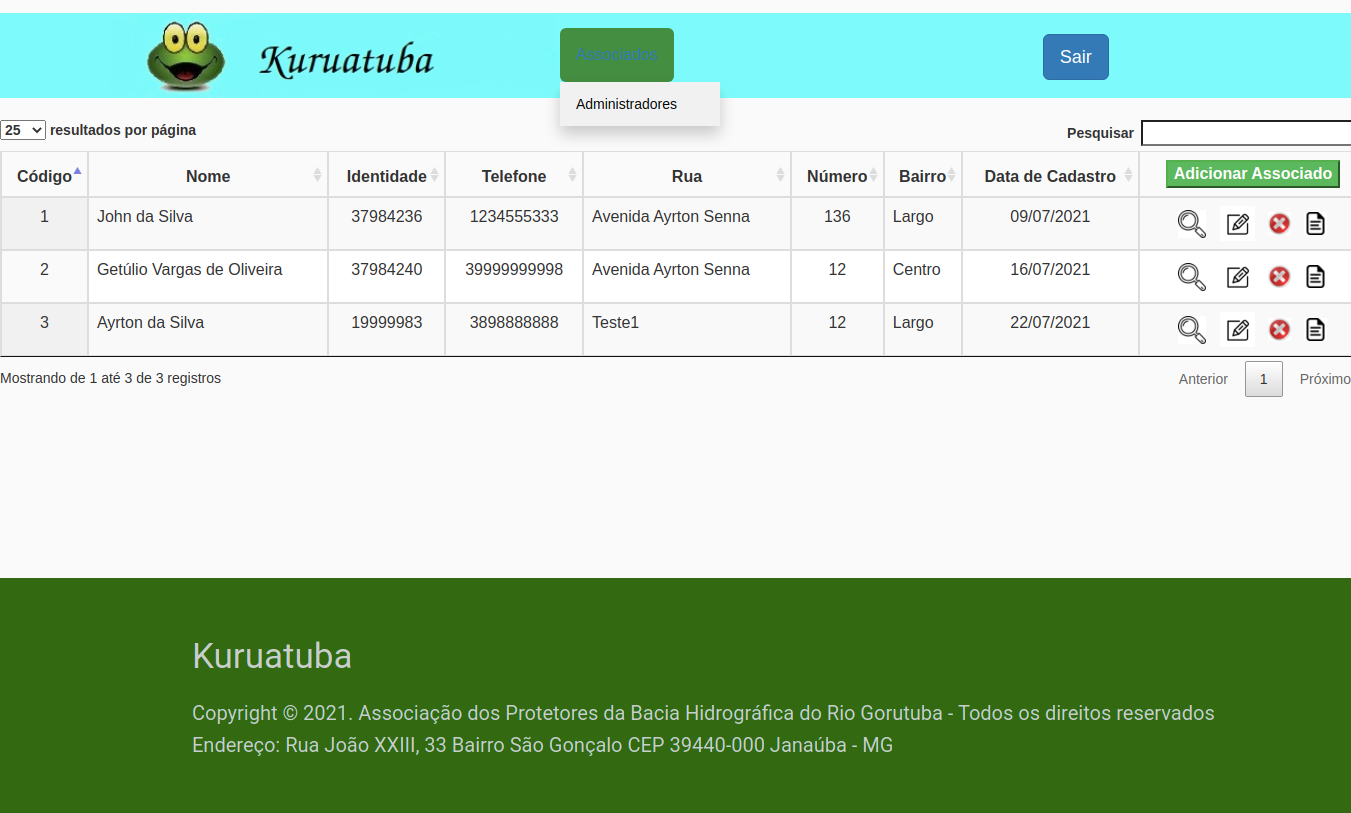
\includegraphics[width=0.9\textwidth]{../figuras/kuruatuba_sistema_home.png}
        \label{fig:home-sistema}
    \end{figure}
\end{frame}



%pag 84
\section{Discussão}
\begin{frame}
    \frametitle{Discussão}
    \begin{itemize}
        \item \textbf{Docker}
        \item \textbf{Git}
    \end{itemize}
\end{frame}


%pag 87
\section{Trabalhos futuros}
\begin{frame}
    \frametitle{Trabalhos futuros}
    \begin{itemize}
        \item Criar manual de utilização do sistema e executar treinamento com futuros usuários;
        \item Instalar um certificado digital (SSL); %em pelo menos as telas de login
        \item Executar testes de software a fim de se obter feedback sobre integridade, disponibilidade e acessibilidade. %Isso é opcional
    \end{itemize}

    
\end{frame}

    

\section{Referências Bibliográficas}

\begin{frame}
    \frametitle{Referências Bibliográficas}
    \tiny{  
        \bibliographystyle{abnt-alf}
        \bibliography{referencias}
    }
  
\end{frame}

\end{document}
